\documentclass[border=4pt]{standalone}
\usepackage{fontspec}
\usepackage{unicode-math}
\setmainfont{texgyretermes}[Extension=.otf, UprightFont=*-regular, BoldFont=*-bold, ItalicFont=*-italic, BoldItalicFont=*-bolditalic]
\setmathfont{texgyretermes-math.otf}
\setsansfont{texgyreheros}[Extension=.otf, UprightFont=*-regular, BoldFont=*-bold, ItalicFont=*-italic, BoldItalicFont=*-bolditalic]
\newfontfamily\tamilfont[Path=../../fonts/, Script=Tamil, BoldFont=NotoSansTamil-Bold.ttf, Scale=0.92]{NotoSansTamil-Regular.ttf}
\newcommand{\ta}[1]{{\tamilfont #1}}
\newcommand{\unk}{\textsc{unknown}}
\usepackage{amsmath,tikz}
\usetikzlibrary{positioning,arrows.meta,shapes,fit,calc,backgrounds}
\begin{document}
% System architecture (Fig. 1)
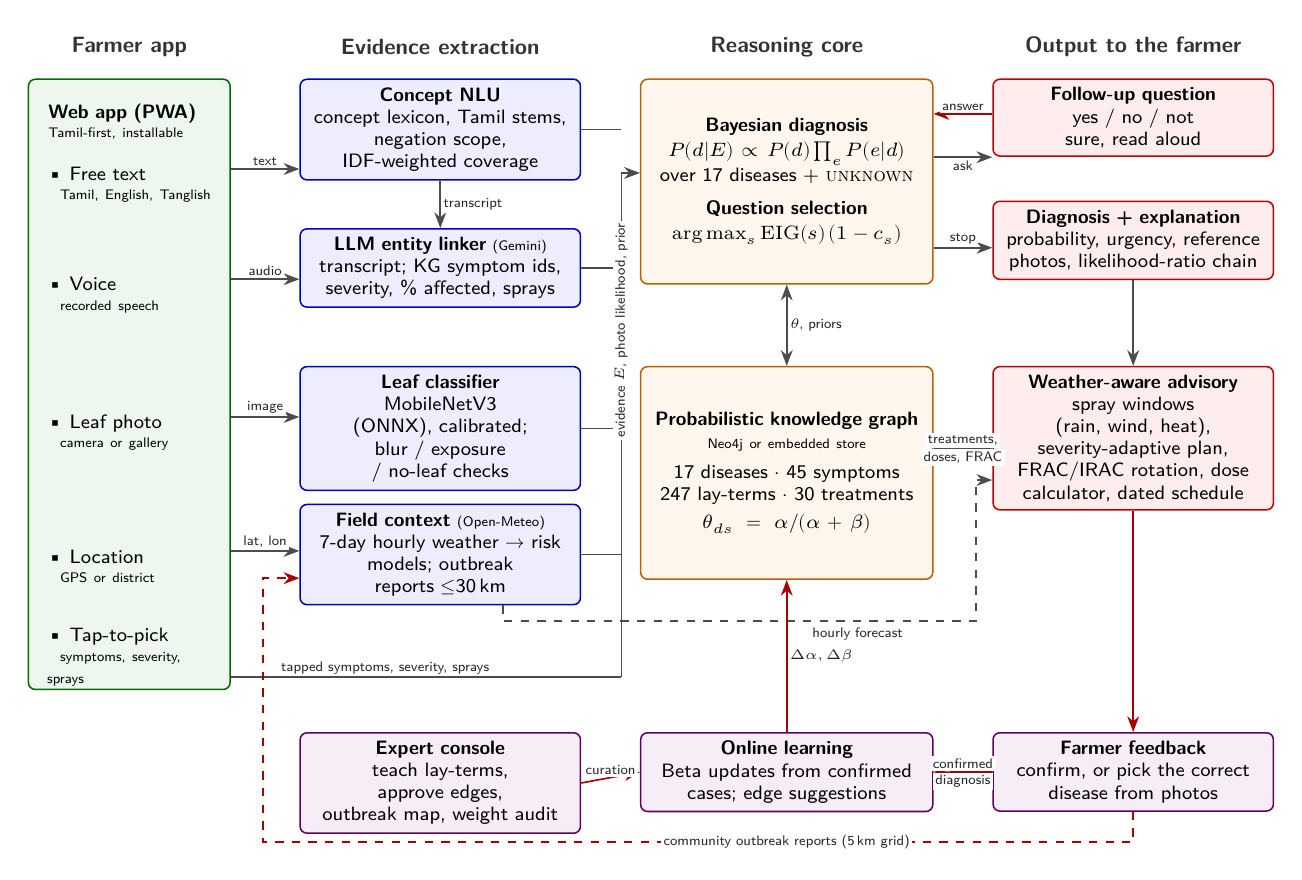
\begin{tikzpicture}[
  font=\sffamily\scriptsize, >=Stealth,
  box/.style={draw=#1!75!black, fill=#1!7, rounded corners=2.5pt, align=center, inner sep=3pt, line width=0.55pt, text width=3.35cm},
  hdr/.style={font=\sffamily\footnotesize\bfseries, align=center, text=black!80},
  flow/.style={->, line width=0.6pt, draw=black!70},
  back/.style={->, line width=0.6pt, draw=red!65!black},
  lbl/.style={font=\sffamily\tiny, fill=white, inner sep=0.9pt, align=center, text=black!85},
]
% ---------------- headers
\node[hdr] at (1.35, 0.55) {Farmer app};
\node[hdr] at (5.3, 0.55) {Evidence extraction};
\node[hdr] at (9.7, 0.55) {Reasoning core};
\node[hdr] at (14.1, 0.55) {Output to the farmer};

% ---------------- inputs (one tall box)
\node[box=green!55!black, text width=2.35cm, minimum height=7.75cm, anchor=north] (in) at (1.35, 0.15) {};
\node[align=left, anchor=north west, text width=2.25cm] at (0.2, -0.05) {\textbf{Web app (PWA)}\\[-1pt]{\tiny Tamil-first, installable}};
\tikzset{inl/.style={align=left, anchor=west, text width=2.2cm, inner sep=0pt}}
\node[inl] at (0.3, -1.2) {\textbullet~Free text\\[-1pt]{\tiny\ \ Tamil, English, Tanglish}};
\node[inl] at (0.3, -2.6) {\textbullet~Voice\\[-1pt]{\tiny\ \ recorded speech}};
\node[inl] at (0.3, -4.35) {\textbullet~Leaf photo\\[-1pt]{\tiny\ \ camera or gallery}};
\node[inl] at (0.3, -6.05) {\textbullet~Location\\[-1pt]{\tiny\ \ GPS or district}};
\node[inl] at (0.3, -7.2) {\textbullet~Tap-to-pick\\[-1pt]{\tiny\ \ symptoms, severity, sprays}};

% ---------------- evidence extraction
\node[box=blue, anchor=north] (nlu) at (5.3, 0.15) {\textbf{Concept NLU}\\ concept lexicon, Tamil stems,\\ negation scope,\\ IDF-weighted coverage};
\node[box=blue, anchor=north] (llm) at (5.3, -1.75) {\textbf{LLM entity linker} {\tiny (Gemini)}\\ transcript; KG symptom ids,\\ severity, \% affected, sprays};
\node[box=blue, anchor=north] (cnn) at (5.3, -3.5) {\textbf{Leaf classifier}\\ MobileNetV3 (ONNX), calibrated;\\ blur / exposure / no-leaf checks};
\node[box=blue, anchor=north] (ctx) at (5.3, -5.25) {\textbf{Field context} {\tiny (Open-Meteo)}\\ 7-day hourly weather $\to$ risk\\ models; outbreak reports $\leq$30\,km};

% ---------------- reasoning core
\node[box=orange, anchor=north, minimum height=2.6cm, text width=3.5cm] (eng) at (9.7, 0.15) {\textbf{Bayesian diagnosis}\\[1pt] $P(d|E)\propto P(d)\prod_{e}P(e|d)$\\ over 17 diseases + \textsc{unknown}\\[4pt] \textbf{Question selection}\\[1pt] $\arg\max_s \mathrm{EIG}(s)\,(1-c_s)$};
\node[box=orange, anchor=north, minimum height=2.7cm, text width=3.5cm] (kg) at (9.7, -3.5) {\textbf{Probabilistic knowledge graph}\\ {\tiny Neo4j or embedded store}\\[3pt] 17 diseases $\cdot$ 45 symptoms\\ 247 lay-terms $\cdot$ 30 treatments\\[2pt] $\theta_{ds}=\alpha/(\alpha+\beta)$};

% ---------------- outputs
\node[box=red, anchor=north] (q) at (14.1, 0.15) {\textbf{Follow-up question}\\ yes / no / not sure, read aloud};
\node[box=red, anchor=north] (dx) at (14.1, -1.4) {\textbf{Diagnosis + explanation}\\ probability, urgency, reference\\ photos, likelihood-ratio chain};
\node[box=red, anchor=north] (adv) at (14.1, -3.5) {\textbf{Weather-aware advisory}\\ spray windows (rain, wind, heat),\\ severity-adaptive plan,\\ FRAC/IRAC rotation, dose\\ calculator, dated schedule};

% ---------------- learning band
\node[box=violet, anchor=north] (exp) at (5.3, -8.15) {\textbf{Expert console}\\ teach lay-terms, approve edges,\\ outbreak map, weight audit};
\node[box=violet, anchor=north, text width=3.5cm] (lrn) at (9.7, -8.15) {\textbf{Online learning}\\ Beta updates from confirmed\\ cases; edge suggestions};
\node[box=violet, anchor=north] (fb) at (14.1, -8.15) {\textbf{Farmer feedback}\\ confirm, or pick the correct\\ disease from photos};

% ---------------- inputs -> evidence
\draw[flow] (in.east |- 0,-1.0) -- node[lbl, above]{text} (nlu.west |- 0,-1.0);
\draw[flow] (in.east |- 0,-2.4) -- node[lbl, above]{audio} (llm.west |- 0,-2.4);
\draw[flow] (in.east |- 0,-4.15) -- node[lbl, above]{image} (cnn.west |- 0,-4.15);
\draw[flow] (in.east |- 0,-5.85) -- node[lbl, above]{lat, lon} (ctx.west |- 0,-5.85);
\draw[flow] (nlu.south) -- node[lbl, right]{transcript} (llm.north);

% ---------------- evidence -> engine (bus)
\def\bus{7.6}
\foreach \n in {nlu, llm, cnn, ctx} \draw[line width=0.6pt, draw=black!70] (\n.east) -- (\bus, 0 |- \n.east);
\draw[line width=0.6pt, draw=black!70] (in.east |- 0,-7.45) -- (\bus, -7.45);
\node[lbl, anchor=south] at (4.6, -7.45) {tapped symptoms, severity, sprays};
\draw[flow] (\bus, -7.45) -- (\bus, -1.05) -- (eng.west |- 0,-1.05);
\node[lbl, rotate=90] at (\bus, -3.05) {evidence $E$, photo likelihood, prior};

% ---------------- core
\draw[flow, <->] (kg.north) -- node[lbl, right]{$\theta$, priors} (eng.south);
\draw[flow] (eng.east |- 0,-0.85) -- node[lbl, below]{ask} (q.west |- 0,-0.85);
\draw[back] (q.west |- 0,-0.3) -- node[lbl, above]{answer} (eng.east |- 0,-0.3);
\draw[flow] (eng.east |- 0,-2.0) -- node[lbl, above]{stop} (dx.west |- 0,-2.0);
\draw[flow] (dx.south) -- (adv.north);
\draw[flow] (kg.east |- 0,-4.55) -- node[lbl, above]{treatments,}node[lbl, below]{doses, FRAC} (adv.west |- 0,-4.55);
\draw[flow, dashed] ([xshift=8mm]ctx.south) -- ++(0,-0.2) -| (12.1, -4.95) -- (adv.west |- 0,-4.95);
\node[lbl] at (10.6, -6.9) {hourly forecast};

% ---------------- learning loop
\draw[back] (adv.south) -- (fb.north);
\draw[back] (fb.west) -- node[lbl, above]{confirmed}node[lbl, below]{diagnosis} (lrn.east);
\draw[back] (lrn.north) -- node[lbl, right]{$\Delta\alpha,\Delta\beta$} (kg.south);
\draw[back] (exp.east) -- node[lbl, above]{curation} (lrn.west);
\draw[back, dashed] (fb.south) -- (14.1, -9.55) -- (3.05, -9.55) |- ([yshift=-3mm]ctx.west);
\node[lbl] at (9.7, -9.55) {community outbreak reports (5\,km grid)};
\end{tikzpicture}

\end{document}
